\documentclass[12pt,preprintnumbers,amsmath,amssymb,nofootinbib,superscriptaddress]{revtex4-1}
\usepackage[paperheight=12cm,top=0.5cm,bottom=0.5cm,left=1cm,right=1cm]{geometry}
\usepackage{xparse}
\NewDocumentCommand{\DIV}{om}{%
  \IfValueT{#1}{\setcounter{#2}{\numexpr#1-1\relax}}%
  \csname #2\endcsname
}

\usepackage[latin1]{inputenc}
\usepackage{slashed}
\usepackage{amsmath}
\usepackage{textcomp}
\usepackage{amssymb}
\usepackage{amsfonts}
\usepackage{indentfirst}
\usepackage{color}
\usepackage[dvipsnames]{xcolor}
\usepackage{hyperref}
\usepackage{subcaption}
\usepackage{graphicx,graphics}
\graphicspath{{figures/}}
\usepackage[skins,theorems,many]{tcolorbox}
\tcbset{highlight math style={enhanced,
  colframe=red,colback=white,arc=0pt,boxrule=1pt}}
\usepackage[abs]{overpic}
\usepackage{xcolor,varwidth}
\usepackage[english]{babel}
\usepackage{blindtext,tikz}
\usetikzlibrary{calc}
\usepackage{fancyhdr}

\def\bibsection{\section*{}} %Removes black line above refrences

%--------------------------%
%----- COLOURED BOXES -----%
%--------------------------%

%Blue equation box
%\tcbhighmath[colframe=RoyalBlue!70!black,colback=RoyalBlue!25!white]{

%Orange equation box
%\tcbhighmath[colframe=BurntOrange!95!black,colback=BurntOrange!45!white]{

%Purple equation box
%\tcbhighmath[colframe=Purple!150!black,colback=Purple!30!white]{

%Green equation box
%\tcbhighmath[colframe=ForestGreen,colback=ForestGreen!25!white]{

%Grey equation box
%\tcbhighmath[colframe=Black,colback=Black!10!white]{

%Pink equation box
%\tcbhighmath[colframe=magenta,colback=magenta!20!white]{

%Blue and red equation box
%\tcbhighmath[frame style={left color=RoyalBlue!70!black,right color=Red!95!black},interior style={left color=RoyalBlue!35!white,right color=Red!50!white}]{

%Red and green equation box
%\tcbhighmath[frame style={left color=Red!95!black,right color=ForestGreen},interior style={left color=Red!50!white,right color=ForestGreen!25!white}]{

\begin{document}

\tikz[overlay,remember picture] % ArXiv number
{
    \node at ($(current page.west)+(1,0)$) [rotate=90] {\Large\textcolor{gray}{arXiv:0000.12345 [hep-th] 30 June 1999}};
}

\pagenumbering{gobble}

\hfill{UK QFT XI/09-01-23} % Conference name and date

\vspace{2.5cm}

\title{
\tcbhighmath[frame style={left color=RoyalBlue!70!black,right color=Red!95!black},interior style={left color=RoyalBlue!35!white,right color=Red!50!white},boxrule=2pt]{
\text{\Large Academic Presentation template}
}}

\author{Drew Backhouse}

\affiliation{Theoretical Particle Physics and Cosmology, King's College London, WC2R 2LS, UK}


\maketitle

\newpage

%-----EXAMPLE SLIDES-----%

\newpage

\DIV[1]{section}{Section 1}\label{Ueff}
\vspace{-0.7cm}
\DIV[3]{subsection}{Subsection A}
\vspace{-0.2cm}\hrule

\vspace{2cm}

\begin{equation}
\tcbhighmath[colframe=Black,colback=Black!10!white]{
Z[j]=
\int\mathcal{D}\varphi \exp\left(-S[\varphi]\right)
}\nonumber
\end{equation}

\vspace{1cm}

\begin{equation}
\tcbhighmath[colframe=ForestGreen,colback=ForestGreen!25!white]{
\text{Sentence of great physical importance}
}\nonumber
\end{equation}

\vspace{\fill}
\centering
\cite{Alexandre:2022sho} J. Alexandre and D. Backhouse (2022)

\newpage

\DIV[1]{section}{Section 1}
\vspace{-0.7cm}
\DIV[2]{subsection}{Subsection B}
\vspace{-0.2cm}
\hrule

\vspace{0.8cm}

\begin{minipage}{0.6\textwidth}
    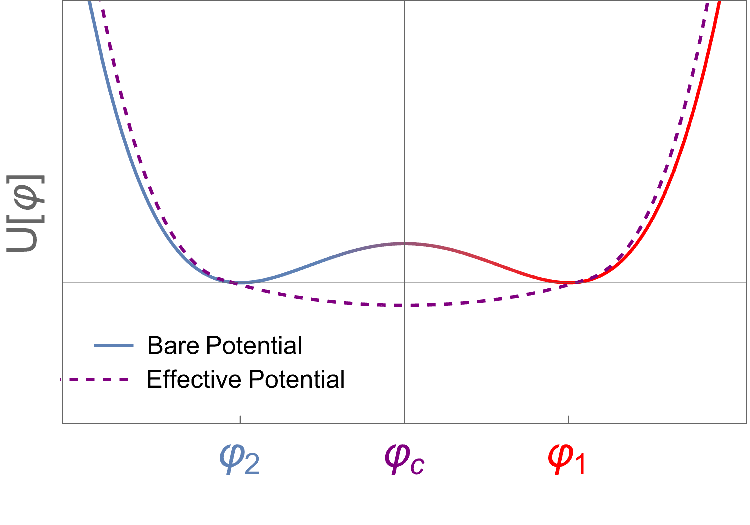
\includegraphics[width=\linewidth]{Figures/EffectivePotential.pdf}
\vspace{-2cm}

\end{minipage}
\begin{minipage}{0.39\textwidth}

\begin{equation}
\tcbhighmath[frame style={left color=RoyalBlue!70!black,right color=Red!95!black},interior style={left color=RoyalBlue!35!white,right color=Red!50!white}]{
U[\varphi]=\frac{\lambda v^4}{24}(\varphi^2-1)^2\nonumber}
\end{equation}

\vspace{1cm}

\begin{equation}
\tcbhighmath[colframe=Purple!150!black,colback=Purple!30!white]{
U_\text{eff}(\varphi_c)=\frac{1}{V\beta}\Gamma[\varphi_c]\nonumber}
\end{equation}

\end{minipage}

\vspace{\fill}
\centering
\cite{Alexandre:2022sho} J. Alexandre and D. Backhouse (2022)

\newpage 

\DIV[2]{section}{References}
\vspace{-0.2cm}\hrule

\bibliography{Bibliography}

\vspace{\fill}
\centering
\href{https://www.overleaf.com/latex/templates/academic-presentation-template/jpgfpsstrwzd}{Template submitted by D. Backhouse}

\end{document}